\subsection{Analysis of Calibration Frames}

The figures below show both the manual and automated calibration frame masks for
three (Figure~\ref{fig:3m_mask_overlays}) and ten (Figure~\ref{fig:10m_mask_overlays})
meters (seen in section~\ref{subsubsec:mask_creation}) superimposed atop their
corresponding raw calibration frame.

Analysis of automated calibration frames, overlays, failure cases, etc

\begin{figure}[htbp]
    \centering
    \makebox[0.8\textwidth][c]{
        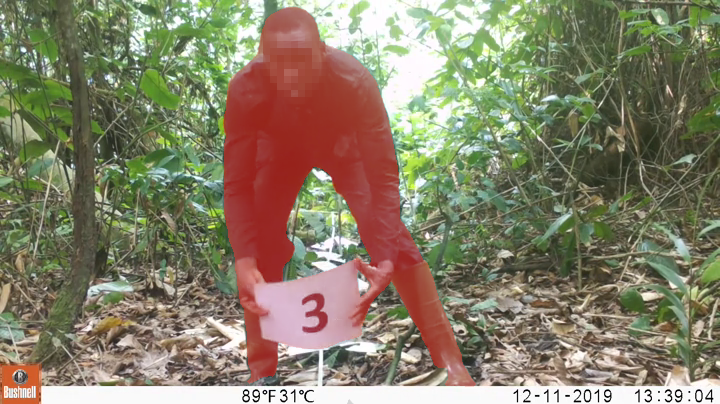
\includegraphics[width=0.9\textwidth]{body/analysis/assets/frame_masks/close_manual_overlay}
    }\\[1mm]
    \makebox[0.8\textwidth][c]{
        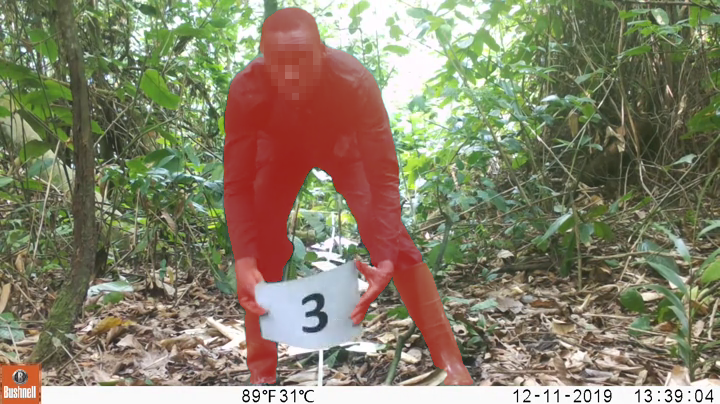
\includegraphics[width=0.9\textwidth]{body/analysis/assets/frame_masks/close_sam_overlay}
    }
    \caption{Three meter manual (top) and automated (bottom) calibration frame segmentation masks overlayed over
    the raw calibration frame}
    \label{fig:3m_mask_overlays}
\end{figure}

\begin{figure}[htbp]
    \centering
    \makebox[0.8\textwidth][c]{
        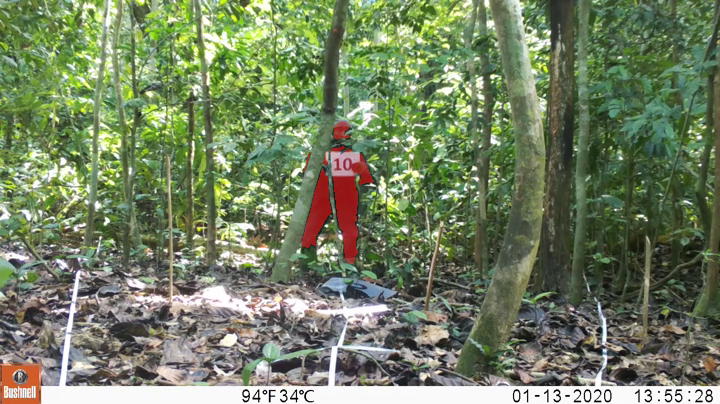
\includegraphics[width=0.9\textwidth]{body/analysis/assets/frame_masks/far_manual_overlay}
    }\\[1mm]
    \makebox[0.8\textwidth][c]{
        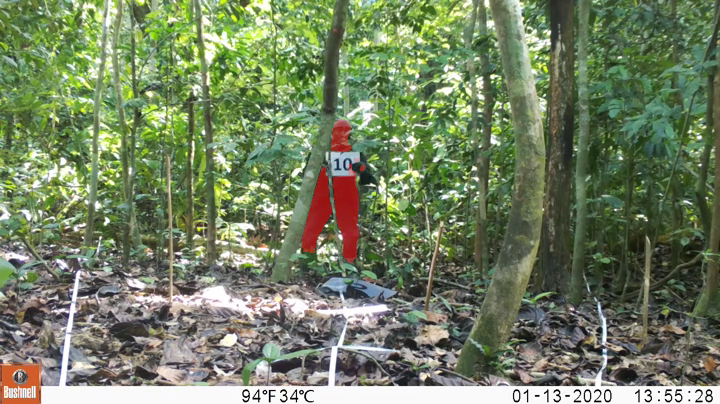
\includegraphics[width=0.9\textwidth]{body/analysis/assets/frame_masks/far_sam_overlay}
    }
    \caption{Ten meter manual (top) and automated (bottom) calibration frame segmentation masks overlayed over
    the raw calibration frame}
    \label{fig:10m_mask_overlays}
\end{figure}